\documentclass[11pt]{article}
\usepackage{graphicx} % Required for inserting images
\usepackage[acronym]{glossaries}
\usepackage{geometry}
\usepackage{biblatex}
\usepackage{hyperref}
\usepackage{wrapfig}
\usepackage{flafter}

 \geometry{
 a4paper,
 left=10mm,
 right=10mm,
 top=5mm,
 bottom=5mm,
 }
 
\title{Deep Learning in Robotic Vision}
\author{Jack Pay}

\newacronym{dl}{DL}{Deep Learning}
\newacronym{dnn}{DNN}{Deep Neural Network}
\newacronym{dnns}{DNNs}{Deep Neural Networks}
\newacronym{cnn}{CNN}{Convolutional Neural Network}
\newacronym{cnns}{CNNs}{Convolutional Neural Networks} 
\newacronym{vit}{ViT}{Vision Transformer} 
\newacronym{nlp}{NLP}{Natural Language Processing}
\newacronym{mha}{MHA}{Multi-Head Attention}
\newacronym{lr}{LR}{Learning Rate}
\newacronym{rmsprop}{RMSprop}{Root Mean Square Propagation}

\addbibresource{refs.bib}

\def\COLABLINK{https://colab.research.google.com/drive/1SfKWE0-IMnT1rEtc4YB5jPUos6SVVEtE?usp=sharing}
\def\BESTWIDTH{256 }
\def\BESTDEPTH{3 }
\def\DATASET{CIFAR100 }
\def\FINALACCURACY{61.130\% }
\def\FINALLOSS{1.977 }

\begin{document}

\maketitle

\section{Literature Review}
Development in \acrfull{dl} has spurred significant progress in various robotics fields, in particular robot vision~\cite{Deep_learning_in_robotics:_a_review}. \acrshort{dnn}s can easily model complex functions without requiring expert knowledge or feature engineering~\cite{Deep_learning_in_robotics:_a_review}. However, numerous challenges persist within this field, such as models' adaptability to spatially and temporally changing environments, something key to robotic vision as opposed with computer vision~\cite{limits_and_potentials_of_deep_learning_for_robotics, An_evaluation_of_EfficientDet}. This review will aim at analysing the state of the art \acrshort{dl} methods for robotic vision, summarising the explosive advancement made in recent years.\\
Classified by their Convolutional layers, Pooling layers, Fully-Connected layers and non-linear activation functions~\cite{Convolutional-neural-network:-a-review-of...}, \acrfull{cnns} are a staple of robot vision~\cite{A-Survey-on-Deep-Learning-Methods-for-Robot-Vision}. Architectures such as AlexNet~\cite{OG_Alexnet}, ResNet~\cite{OG_resnet} and EfficientNet~\cite{OG_EfficientNet} have revolutionised robotic vision, allowing significant advancement in performance throughout the past few decades.\\
In 2012, Krizhevsky et al. developed AlexNet~\cite{OG_Alexnet}, a \acrshort{cnn} architecture that achieved state of the art performance in image classification at that time and won the ImageNet LSVRC-2010 competition~\cite{OG_Alexnet}. AlexNet was made distinct by its use of dropout, a regularization method used to randomly omit hidden units from the training process~\cite{OG_dropout}. Counter-intuitively, this prevents overfitting~\cite{Avoiding_overfitting...} and produces models that generalize better~\cite{regularization}. This is because it forces hidden units to not always rely on the prescence of other specific units~\cite{OG_dropout}. AlexNet also utilised a convolution implementation specifically produced to take advantage of GPUs and accelerate training~\cite{OG_Alexnet}.\\ 
Winning the ILSVRC-2015 classification task, ResNet was developed in 2015 by He et al.~\cite{OG_resnet}. Similarly to AlexNet, this \acrshort{cnn} for image classification was trained and evaluated upon the ImageNet dataset but owed its success to the ``Residual connections" employed throughout its architecture. Residual connections are a type of shorcut, or skip connection, where the output of a hidden layer is combined with the original input to that layer~\cite{OG_resnet}. This makes \acrshort{dnn} significantly easier to train as it reduces the vanishing gradient problem~\cite{ResNet:_Solving_Vanishing_Gradient...} and therefore improves training and test loss~\cite{Demystifying_ResNet}.\\
However, a primary downside of \acrshort{cnn} architectures for robotics at this time was the size of models produced~\cite{Trends_in_deep_convolutional_neural_Networks}. The size of models and, therefore, speed of inference is a crucial factor within robot vision~\cite{future_trends_on_robot_vision_technology}, where a difference of seconds could result in or prevent human injury.\\
Developed in 2019 by Tan et al., EfficientNet~\cite{OG_EfficientNet} was a \acrshort{cnn} that addressed this issue. EfficientNet employed a method called ``compound coefficient" for scaling the size of the \acrshort{dnn} ( in terms of width, depth and resolution) based on the size of the input~\cite{OG_EfficientNet}. Compound coefficient was massively successful for developing an architecture not only with state of the art performance but also computational efficiency and improved model size, being able to run within even smaller, less powerful devices~\cite{An_evaluation_of_EfficientDet, L-EfficientUNet:_Lightweight_End-to-End}. EfficientNet also boasted further, faster training times~\cite{Efficientnetv2}, a quality useful for incremental learning within robotics~\cite{limits_and_potentials_of_deep_learning_for_robotics}.\\
Predominantly employed within the field of \acrshort{nlp}~\cite{A_survey_of_visual_Transformers, Transformers_in_vision:_A_survey}, transformer architectures have also shown great success in the field of robotic vision~\cite{Real-world_robot_learning_with_masked_visual_pre-training}. Examples of architectures include the original \acrfull{vit}~\cite{OG_vit}, the Visual Saliency Transformer~\cite{Visual_saliency_Transformer} and Contextual Transformer~\cite{contextual_Transformer}.\\
Transformer architectures boast several advantages when compared to other methods: from their state of the art performance yet smaller computational cost~\cite{OG_vit}, to requiring fewer prior assumptions or inductive biases prior to training~\cite{Transformers_in_vision:_A_survey}. Fine-tuning pretrained models, rather than training one from scratch, reduces the amount of data and effort required for training transformers~\cite{Monocular_Robot_Navigation...}. A major part of robotics, vision or otherwise, is incorporating and utilising data of different modalities~\cite{Learning_Unseen_Modality_Interaction}. Transformers are able to easily extend and incorporate different modalities~\cite{Transformers_in_vision:_A_survey} such as combining both visual and proprioceptive senses for improved locomotion~\cite{Learning_Vision_Guided_Quadrupedal_Locomotion...}.\\
In summary, \acrshort{dl} is the state of the art method for robotic vision. \acrshort{cnn}s and transformers are intrinsic to robotic vision, addressing robotic's crucial requirements for accuracy, speed and efficiency~\cite{limits_and_potentials_of_deep_learning_for_robotics, future_trends_on_robot_vision_technology}.

\section{Introduction}
Note that all experimentation was conducted within the notebook found here: \url{\COLABLINK}.\\
This experimentation aimed at finding a high performance \acrshort{dnn} architecture for image classification, therefore researching robotic vision. For this aim, the \DATASET~\cite{cifar100} dataset was employed due to its easy accessibility, free usage, complexity and size. This dataset poses a higher level of complexity compared with CIFAR10~\cite{cifar100}, whilst \DATASET involves classification of 100 classes, rather than just 10. All images within the CIFAR datasets are 32x32 pixels in size and have 3 colour channels. Not that other than normalisation, little preprocessing was carried out on this dataset.\\
In total, sixteen experiments were conducted experimenting with the architecture of \acrshort{cnn}s, their structure being the primary experimental hyperparameter. Experiments varied the components used within the model architecture, trialing the added benefit of Residual connections and \acrfull{mha}. Furthermore, investigation into the network's width and depth was carried out. The methodology involved utilising KerasTuner~\cite{kerastuner} to carry out a quadratic grid based search upon the number of units within each Convolutional layer and the number of Residual blocks in the network, simultaneously.\\
\section{Approach}
Presented within Table~\ref{table: All Experiments} is a summary of the major experiments conducted within this research.\\
Each of the experiments utilised a \acrfull{lr} of 0.0001 (allowing slow convergence towards the optimal) and trained for 100 epochs, allowing for models to reach an optimum. The \acrfull{rmsprop} optimization algorithm was also employed to tune the \acrshort{lr} throughout training and to circumvent under and overfitting. \DATASET consists of 10,000 test data samples, set aside for final evaluation of each trained model, and 50,000 training samples. These training samples were then split: 80\% being set aside for training and the remaining 20\% for validation. The validation set was utilised to evaluate the performance of and tune the hyperparameters of the networks throughout training.\\
Firstly a basic \acrshort{cnn} architecture consisting of Convolutional layers, Max-Pooling layers and a Fully-Connected final layer was trained to serve as a baseline for the experimentation. Next, for the second experiment, this architecture was adapted: after a first plain \acrshort{cnn} block, Residual blocks were used. These consisted of Convolutional + Activation + Batch Normalisation + Convolutional + Add + Activation + Batch Normalisation + Max Pooling, where the Add layer summed the original input with the hidden representation from the previous layer. Experiment three integrated a \acrshort{mha} block into the base \acrshort{cnn} architecture. The \acrshort{mha} blocks consisted of \acrshort{mha} + Add + Layer Normalisation, where the Add layer summed the original input and output from the Attention layer. Next, the fourth experiment utilised a combination of the architectures from the previous two experiments: both the Residual and \acrshort{mha} blocks were added into a \acrshort{cnn}, further boosting the performance for image classification.\\
The fifth experiment used KerasTuner's GridSearch~\cite{kerastuner} to run twelve individual experiments, varying the width of the Convolutional layers and the number of Residual blocks. The values [32, 64, 128, 256] and [1,2,3] were employed respectively, changing the width and depth of the network. These experiments involved training the models for just twenty epochs and with a \acrshort{lr} of 0.0001 to find the optimal model architecture. This number of epochs was a compromise between saving resources and ensuring reliability of the experiment. The result of these twelve experiments revealed the best width to be \BESTWIDTH Convolutional units and the best depth to be \BESTDEPTH Residual blocks.\\
Once the fifth experimentation had concluded, the best hyperparameters were employed to train a final model. This model was further optimised using Exponential \acrshort{lr} scheduling, some minor Data Augmentation and Early Stopping. The effect of this was further boosted performance and reduced overfitting.

\begin{table}
\centering
\begin{tabular}{|c|p{80mm}|c|c|} 
 \hline
 Experiment & Summary &  Testing Accuracy & Testing Loss \\ [0.2ex] 
 \hline
 1 & Basic \acrshort{cnn} & 34.960\% & 2.560 \\
 \hline
 2 & \acrshort{cnn} with Residual connections & 47.480\% & 2.056 \\
 \hline
 3 & \acrshort{cnn} with \acrshort{mha} & 46.900\% & 2.123 \\
 \hline
 4 & \acrshort{cnn} with Residual connections and \acrshort{mha} & 49.030\% & 1.969 \\
 \hline
 5 & \acrshort{cnn} with Residual connections and \acrshort{mha}. Varied size of the Convolutional layers with the values [32, 64, 128, 256] and varied the number of Residual blocks with the values [1,2,3] & (Best) 57.410\% & (Best) 3.394 \\
 \hline
 6 & \acrshort{cnn} with Residual connections and \acrshort{mha}. Exponential \acrshort{lr}, Data Augmentation and Early Stopping were used &  \FINALACCURACY & \FINALLOSS \\
 \hline
\end{tabular}
\caption{A description of each experiment presented with their test accuracy and loss. Note that for experiment 5, twelve experiments were conducted. Documented above are the metrics for the best architecture found.}
\label{table: All Experiments}
\end{table}
\section{Evaluation}
\setcounter{figure}{1}
\begin{figure}
  \centering
  \begin{minipage}[t]{0.45\textwidth}
    \centering
    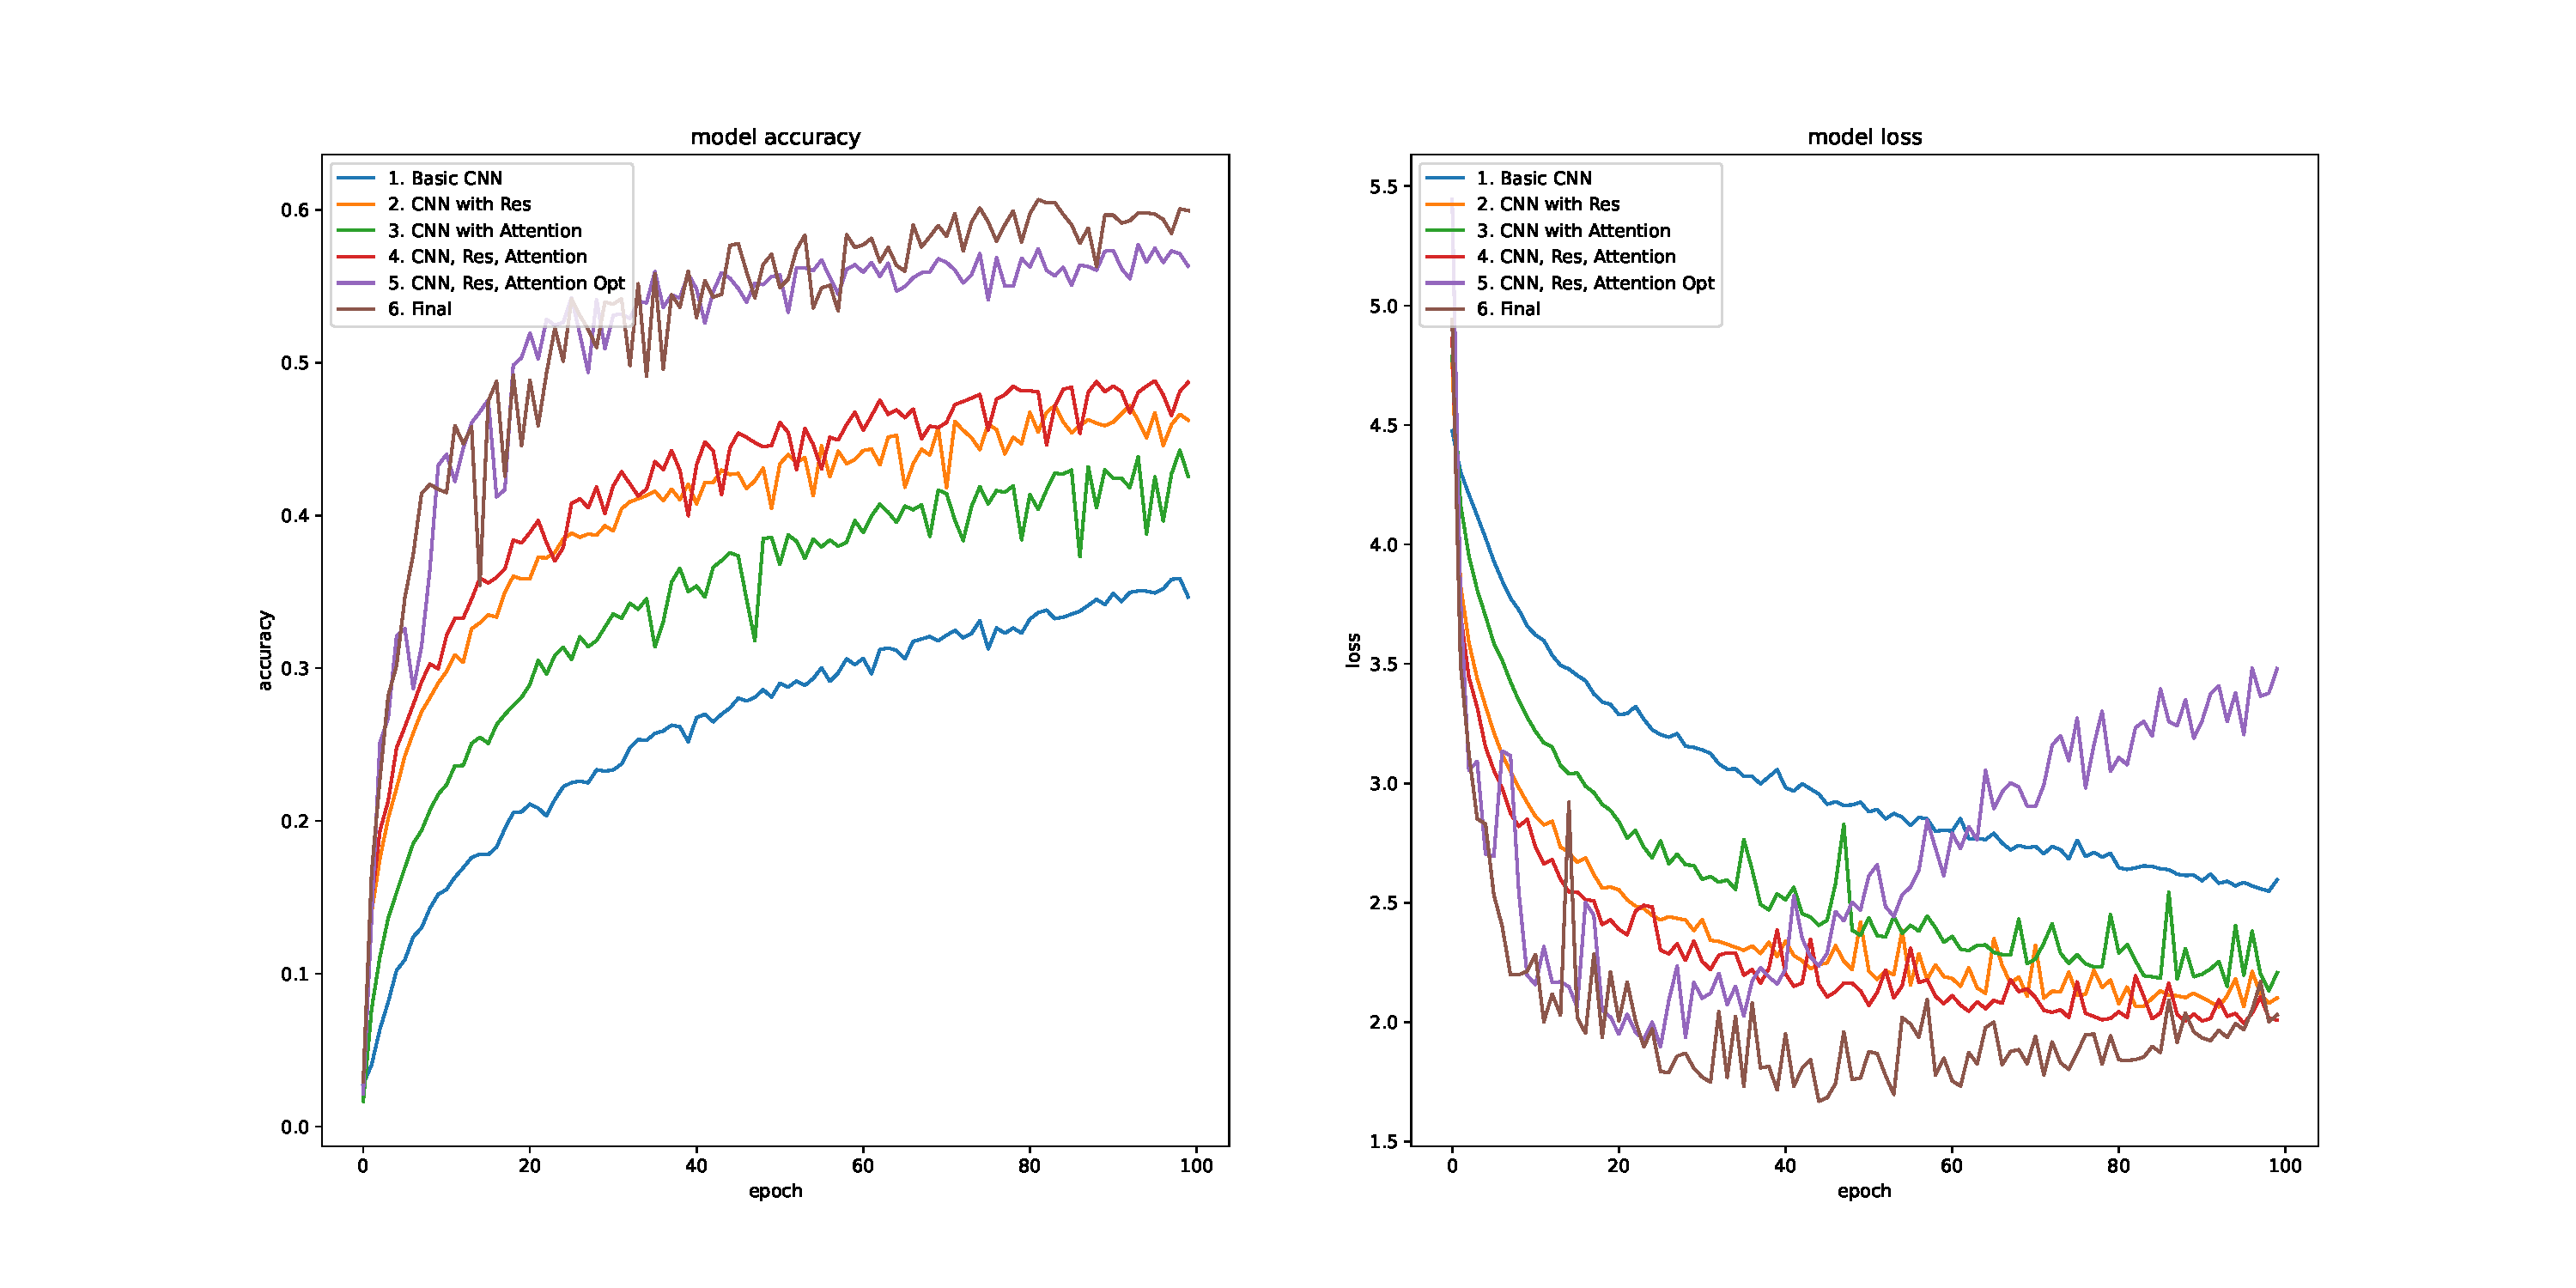
\includegraphics[width=\textwidth]{Figures/all_experiments.pdf}
    \caption{The different major architectures. Experiment 1 used a basic \acrshort{cnn}, 2 a \acrshort{cnn} with Residual connections and 3 a \acrshort{cnn} with \acrshort{mha}. Experiment 4 consisted of a \acrshort{cnn} with 32 wide Convolutional layers, 2 Residual blocks and a \acrshort{mha} block. Experiment 5 and 6 here consisted of a \acrshort{cnn} with \BESTWIDTH wide Convolutional layers, \BESTDEPTH Residual blocks and a \acrshort{mha} block. Experiment 6 was a further optimised model, utilising methods such as Exponential \acrshort{lr} scheduling to reduce overfitting.}
    \label{fig: Major Experiments}
  \end{minipage}
  \hfill
  \begin{minipage}[t]{0.45\textwidth}
    \centering
    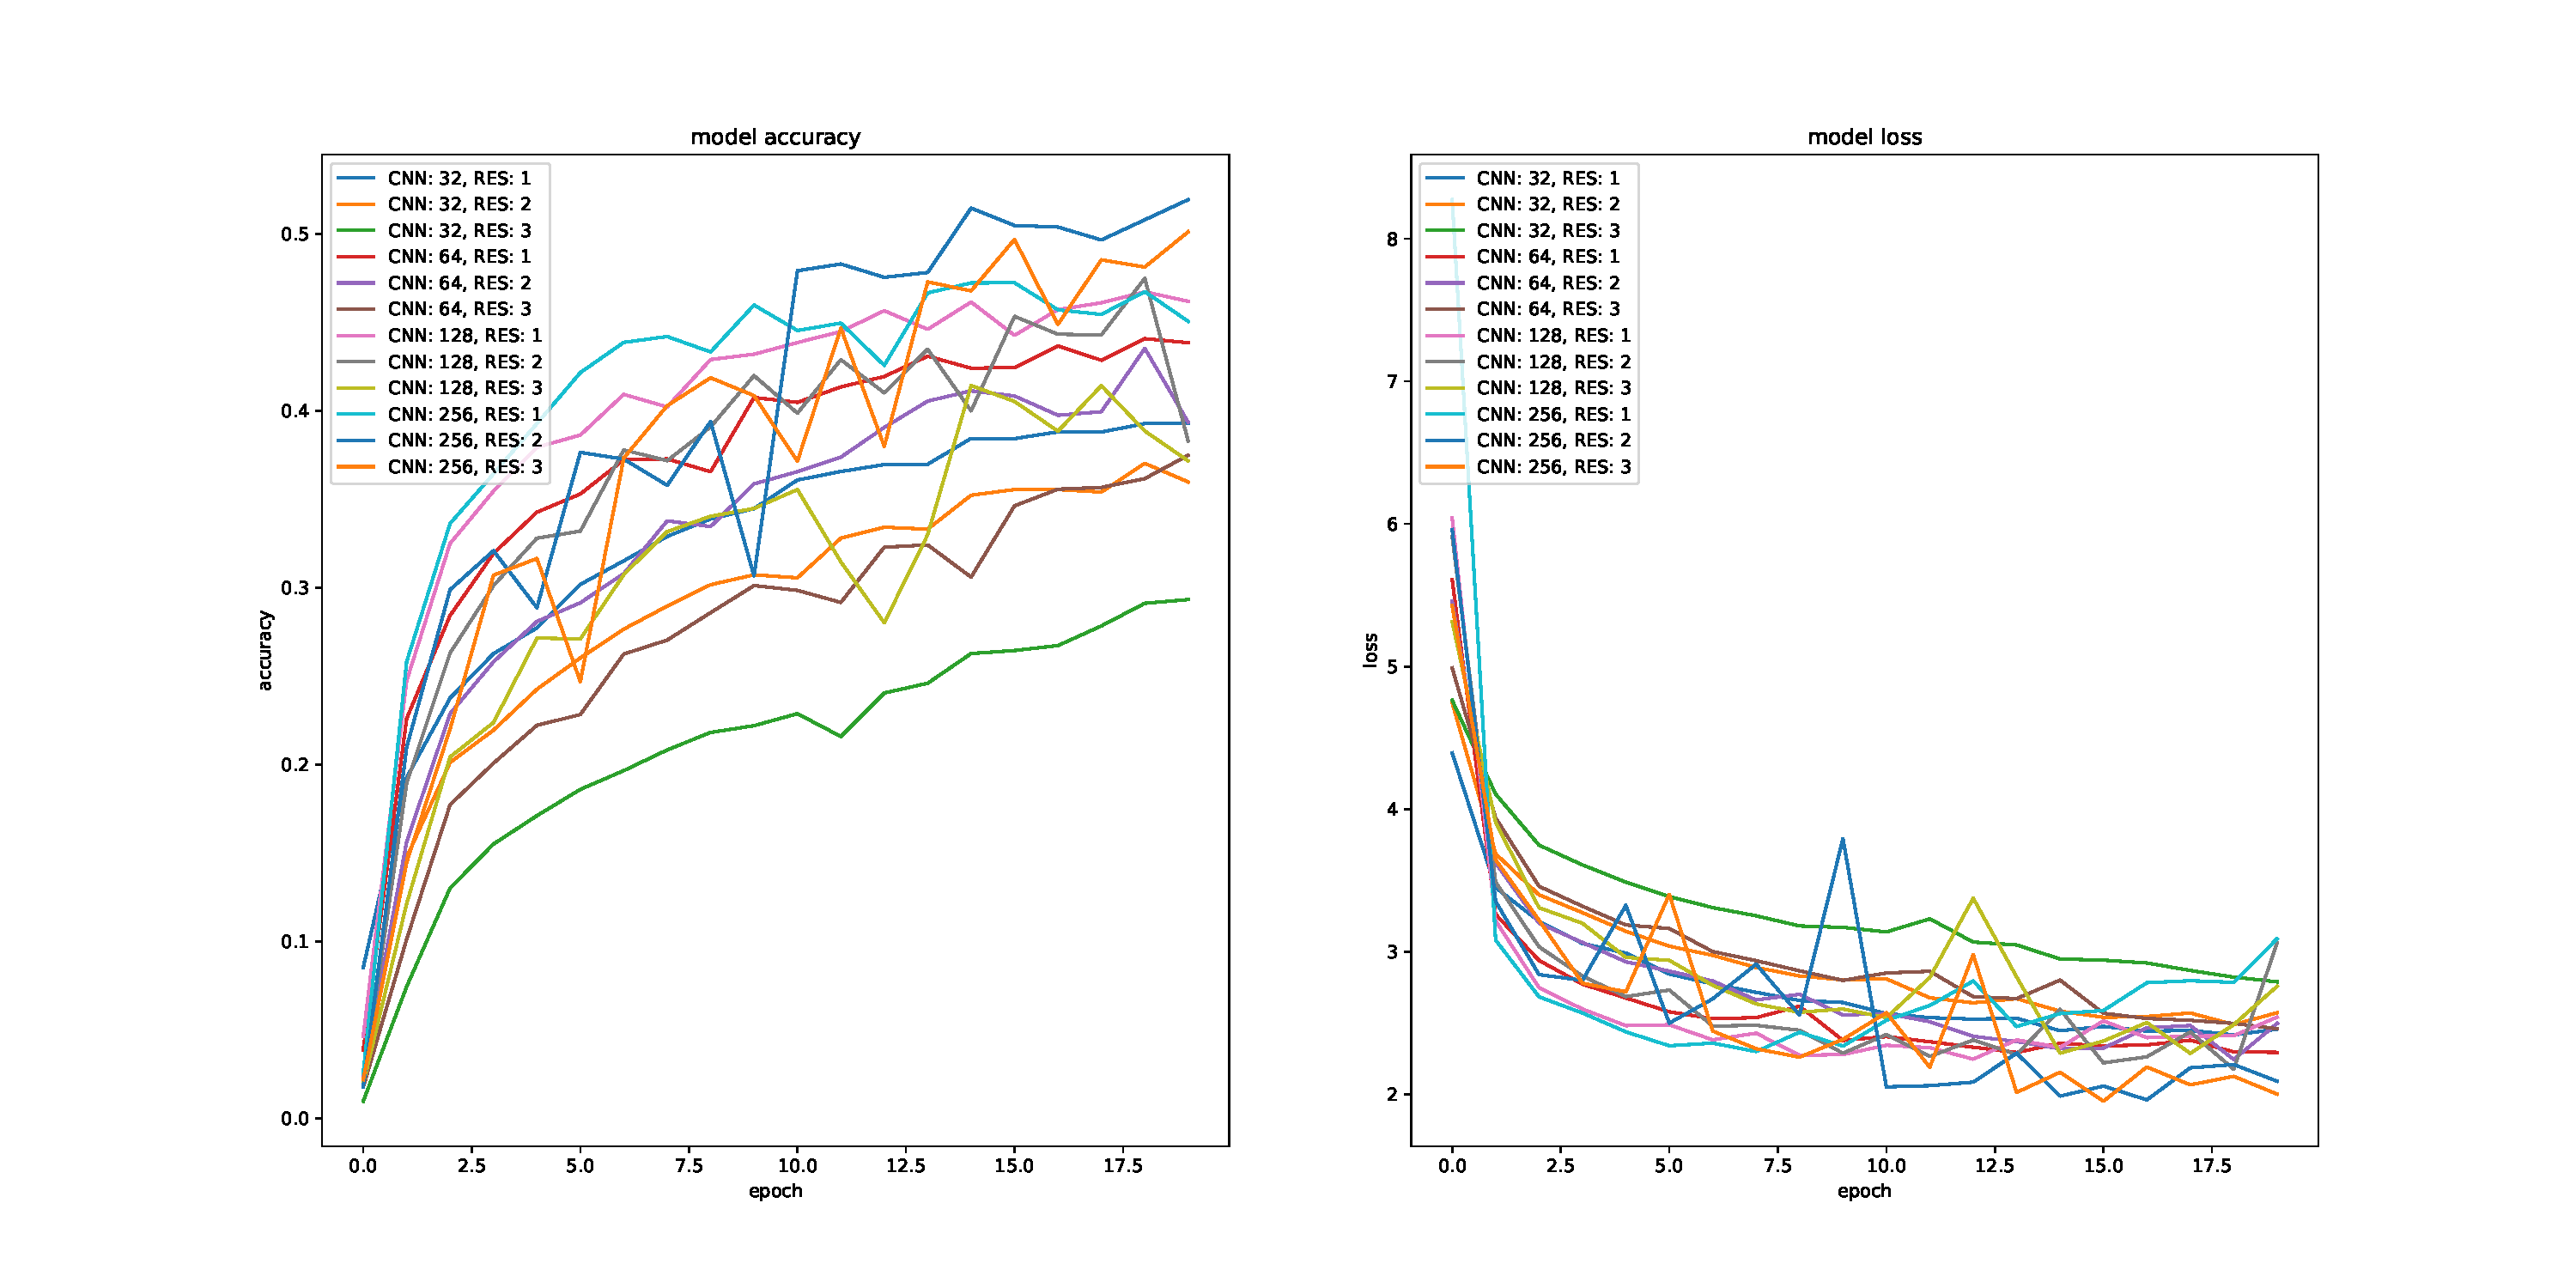
\includegraphics[width=\textwidth]{Figures/experiment_5_trials.pdf}
    \caption{The effect of different widths and depths on the validation accuracy and loss of the model architecture. Here the size of the Convolutional layers and the number of Residual blocks were varied using the values [32, 64, 128, 256] and [1,2,3] respectively.}
    \label{fig: Size Experiment}
  \end{minipage}
\end{figure}
This section will carry out further, detailed evaluation of the results from each of the experiments.\\
Shown in Figure~\ref{fig: Major Experiments}, are the primary experiments. Experiments 1--4 involved modifying the \acrshort{cnn} architecture. Both adding the Residual and \acrshort{mha} blocks improved performance of the \acrshort{cnn} architecture, the former providing a larger increase than the latter. These conclusions are well-trodden: the benefit of skip-connections being evident through ResNet~\cite{OG_resnet, ResNet:_Solving_Vanishing_Gradient...} and Attention through Transformers~\cite{A_survey_of_visual_Transformers, OG_vit}. The Residual connections allow further information to be propagated throughout the network, reducing the vanishing gradient problem and increasing performance. The addition of Attention allows the model to select more important aspects of the image, mirroring animal vision.\\ 
Potentially more interesting is experiment 5 and the results of the twelve experiments upon the size of the model architecture, shown in Figure~\ref{fig: Size Experiment}. Interestingly, the size of the architecture makes a huge impact on the performance of the architectures. A smaller width of network, such as using 32 units within each Convolutional layer results in far lower performance and slower convergence towards an optimal model. This width results in a model that plateaus in performance around 48\% accuracy. But using a wider network, such as up to 256 units per layer, creates a model with improved performance and faster convergence, despite the increased number of network parameters. However, models of this size present a double-edged sword. The longer these larger models are trained, the more they can tend to overfit. This can even result in a decrease in overall performance: the neural network becoming so focused on the training data that the validation loss greatly worsens. This is evident in Figure~\ref{fig: Major Experiments}: after approximately 20 epochs, experiment 5 increase in loss again, becoming one of the most accurate models but also the one with the highest loss.\\
The primary reason for this is the time taken for convergence and the \acrshort{lr} scheduling. The smaller networks took a long time to converge, barely reaching a plateau in performance by the end of the hundredth epoch. However, the larger models quickly increase in performance, possibly faster than the \acrshort{lr} scheduler can keep up. The \acrshort{lr} is still too high at this point, resulting in overfitting.\\
From experiment 5, the optimal hyperparameters, of \BESTWIDTH Convolutional units and \BESTDEPTH Residual blocks, were discovered. This provided the lowest loss of any of the twelve experiments. From these findings it was also discovered that the width of the neural network made a far more significant impact compared with the depth. Varying the number of Residual blocks in a row would have different impacts of the performance: sometimes increasing accuracy and other times decreasing it. Overall, the number of units in each convolutional layer made a far larger and consistent impact. This is useful for finding a smaller neural network for robotic vision. It may be better to prioritse the width rather than depth or even find a suitable balance between the two whilst speed and size of such models is a crucial in robotics.

\subsection{Optimal Hyperparameters}
\begin{figure}
\centering
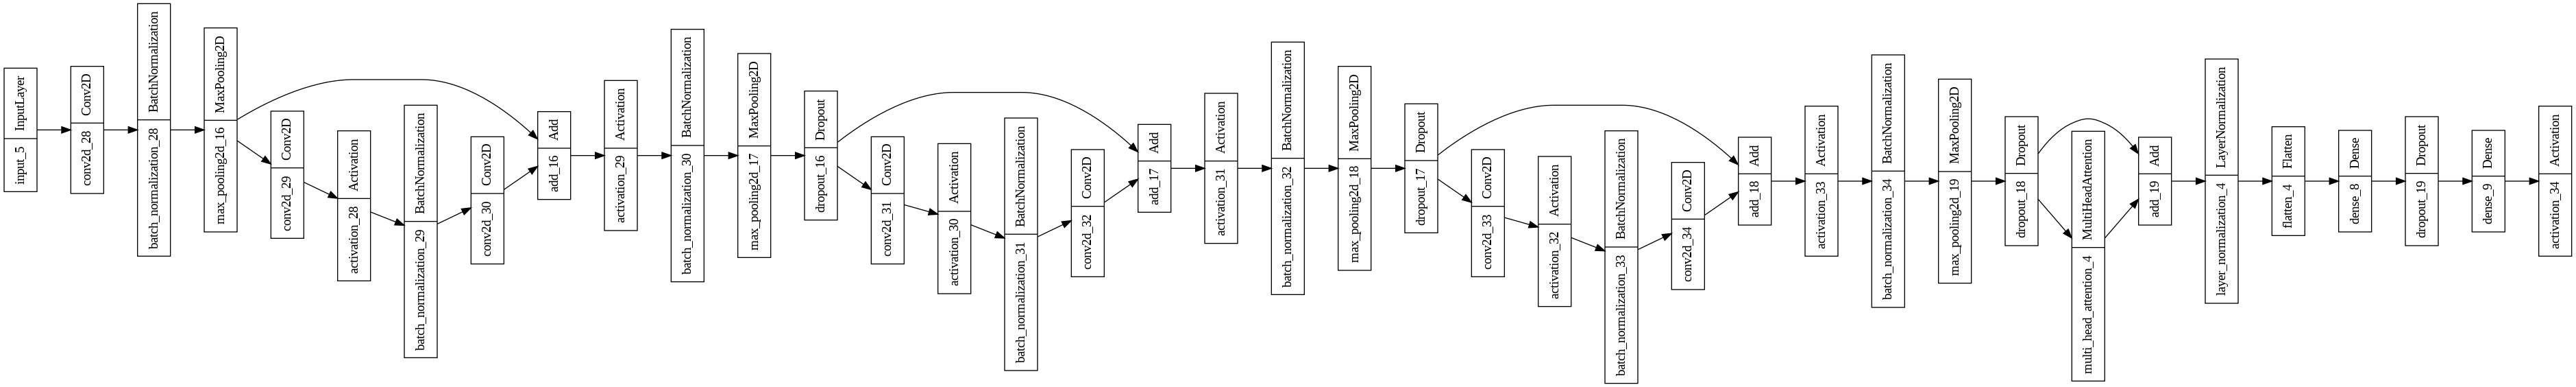
\includegraphics[width=0.9\textwidth]{Figures/experiment_6_arch.png}
\caption{The architecture of the final model. This is a \acrshort{cnn} with Residual connections and \acrfull{mha}. Convolutional layers contain \BESTWIDTH units and the architecture contains \BESTDEPTH main Residual blocks.}
\label{fig: Final Architecture}
\end{figure}
\setcounter{figure}{0}
\begin{wrapfigure}{r}{0.5\textwidth}
\centering
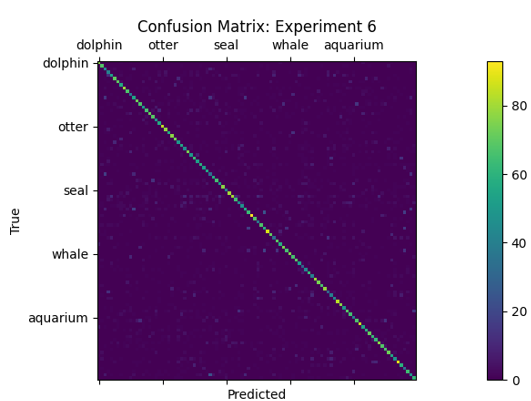
\includegraphics[width=0.5\textwidth]{Figures/Final_Confusion_Matrix.png}
\caption{A confusion matrix of the final model's performance on the \DATASET test dataset. This \acrshort{cnn} was composed of Connvolutional layers with \BESTWIDTH units, \BESTDEPTH Residual blocks followed by a \acrshort{mha} block with 3 heads. This architecture achieved an accuracy of \FINALACCURACY and loss of \FINALLOSS.}
\label{fig: Confusion Matrix}
\end{wrapfigure}
With the findings from the previous experiments, a final model was then trained. The architecture for this model is presented within Figure~\ref{fig: Final Architecture}. This model utilised the best hyperparameters of \BESTWIDTH Convolutional units and \BESTDEPTH Residual blocks.  Both the Residual blocks and \acrshort{mha} block were incorporated into this architecture.\\
Furthermore, with the findings from experiment 5, surrounding overfitting of such a large model, a second \acrshort{lr} scheduling method of Exponential Decay was utilised. Whilst \acrshort{rmsprop} algorithm was previously used to adapt the \acrshort{lr} throughout training, this was found to not be enough. Therefore Exponential Decay was also employed to decrease the overall \acrshort{lr} at regular intervals. With this method, every epoch the \acrshort{lr} was multiplied by $e^{-0.99}$, to ensure further stability within the training process. To balance the fast momentum of this scheduling, a higher initial \acrshort{lr} of 0.001 was employed.\\
This resulted in a final model that plateaued with a higher test accuracy and lower loss of \FINALACCURACY and \FINALLOSS. Rather than overfitting after 20 epochs, the model continued to learn the structure of the data.\\
Whilst the performance of the final model is good for such a complex and high dimensional classification problem, it could still further be improved. Therefore, an extensive confusion matrix was generated, presented within Figure~\ref{fig: Confusion Matrix}. This shows a summary of the performance of the final model on the \DATASET dataset. This was produced to further analyse potential difficulties the model faced, with the aim of suggesting possible future improvements.\\
Some of the \DATASET classes achieved a high F1 score, such as the Beaver class with 0.832 or Apples class with 0.875. However, other classes achieved quite a low performance, possible therefore being responsible for the overall lower performance of this model. Examples include the Girl class with an F1 score of 0.291 or the Camel class with an F1 score of 0.312.\\
A primary reason for this low score could be related to the data distribution and image quality for these classes. For example, other than the Girl class there are several alternative human related classes within \DATASET, such as Woman, Man and Boy. Both Woman and Man share a similarly low F1 score of 0.440. It may be that the data samples belonging to each of these classes are quite similar, making it harder for the model to draw a valid separation between what is a Girl and what is a Woman. Context clues such as wrinkles, face size or clothes may be difficult to make out in the low resolution images. The Camel class' low metrics could also further support this claim, whilst Camel samples might be quite similar to Cattle or even Lion samples. These are all quadrupedal, tan coloured animals, after all.\\

\subsection{Future Work}
Firstly, this research could be taken further, experimenting with wider and deeper \acrshort{cnn} architectures. Here the limit of 256 units was used for the Convolutional layers, however this size could be further expanded. 512 or 1024 units could be trialled to assess their performance also. This research was limited by time, cost and computation power making it infeasible to trial architectures of such sizes.\\ Furthermore, different combinations of widths could be trialed. Here each Residual block was the same width, having Convolutional layers with the same number of units. Instead, different combinations could be tried to see, for example, if a network with a narrow front and wide end is beneficial. This would exponentially add complexity, requiring an even longer search algorithm.\\
This research found that larger networks performed better, but this is maybe harmful to robotic vision. As mentioned within the earlier sections, the size and speed of robotic vision models is crucial, with slow models potentially causing financial damage or harm to humans. Further work could explore the speed of the models presented here, looking to better balance the efficiency of models and the time required for inference.\\
Another improvement of this work could be to better visualise how the model distributes and separates classes, employing methods such as T-distributed Stochastic Neighbor Embedding. Currently, analysis of the final model is mostly speculative and therefore could be further enhanced with sufficient proof of how the model represents samples within the high dimensional, semantic space. This could help to focus on which classes potentially require more data or which features are crucial for separating the data samples.\\
Most investigation here focused on Residual connections and making a \acrshort{cnn} of different sizes. Future work could also expand on the other elements introduced within this work, aiming to exploit them and improve performance overall. \acrfull{mha} was employed in experiment 3, increasing performance of image classification but otherwise, this method was not touched upon greatly, due to time constraints and an already quite complex optimisation task. Different numbers of \acrshort{mha} heads could be trialed or Attention at different points throughout the network could be attempted. Selective attention is a major part of human and robotic vision, therefore further focus on this could be beneficial.\\
Finally, whilst it poses many benefits, the \DATASET dataset is also not perfect. This dataset contains mostly quite simple images, with a single target in frame and clear, complete images. The real world is far noisier than this, with multiple potential target in view at the same time or peculiar poses. Robot vision must be able to cope with these different perspectives and understand how to better orient themselves, or an object being viewed, to maximise performance. Therefore a different, harder dataset such as COCO~\cite{COCO} could be trialed instead.

\renewcommand*{\bibfont}{\tiny}
\printbibliography
\end{document}
